\PassOptionsToPackage{sols}{handout}
\documentclass[main]{subfiles}
\setcounterrefbeforedot{chapter}{m-ws5-5}
\setcounterrefafterdot{section}{m-ws5-5}
\addtocounter{section}{-1}
\usepackage{solutions}

\begin{document}

\ifSubfilesClassLoaded{%
  \chaptermark{\chapterfive}
}{}

\section{The Fundamental Theorem of Calculus, Part 1} \label{ws5-5}

\begin{problemonly}
    \begin{framed}

\textbf{Key Ideas}:

\begin{itemize}[topsep=0pt,partopsep=0pt,parsep=8pt,itemsep=0pt]

\item You should understand and be able to apply Part 1 of the Fundamental
  Theorem of Calculus (FTOC 1), which says that $A'(x) = f(x)$.

\item You should be able to explain why FTOC 1 makes perfect sense when
  $f$ is a rate function.

\item You should understand FTOC 1 from the signed area perspective.

\item You should be able to sketch an area function $A$ given a
  formula or graph of $f$ and an anchor point.
  In particular, you should be able to determine
  where $A$ is increasing/decreasing, concave up/concave down, as
  well as roughly where its intercepts are (there is one intercept you
  should be able to find exactly). 

\end{itemize}
\end{framed}
\end{problemonly}

Last time, we defined the area function (and the 
accumulated amount
function if $f$ is a rate) $A(x)$ by
  $\displaystyle A(x) = \int_a^x f(t)\,dt$ for some anchor point $a$.
  Today, we're going to
  focus on the derivative of this function.

\begin{enumerate}
\item 
  \note{This is essentially identical to {{{{\#4}} on {the worksheet ``Properties of the Definite Integral, The Area Function''}}}.}

  Suppose $f(t)$ represents the rate at which water is flowing into or
  out of a pool at time $t$, where $t$ is measured in hours after
  noon.  At 2 pm, there are 10,000 gallons of water in the pool.
  \begin{enumerate}
  \item
    \begin{problem}[\vfill]
      How much water is in the tank at 5 pm?  Your answer should involve a
      definite integral.
    \end{problem}

    \begin{solution}
      At 2 pm, there are 10,000 gallons of water.  The net change in the
      amount of water from 2 pm to 5 pm is $\displaystyle \int_2^5
      f(t)\,dt$.  So, the amount of water at 5 pm is $\boxed{10000 +
        \int_2^5 f(t)\,dt}$. 
    \end{solution}

  \item

    \note{Often, students want to treat times before the ``anchor point''
      (the $a$ in ${}_a A(x)$) differently from times after the anchor
      point.  This is just an opportunity to discuss why that's not
      necessary.}

    \begin{problem}[\vfill]
      How much water is in the tank at 1 pm?
    \end{problem}

    \begin{solution}
      This is just like {{{{\#1}}(a)}},
      except that we want to know what happens at 1 pm instead of 5 pm;
      the amount at 1 pm is $\boxed{10000 + \int_2^1 f(t)\,dt}$.

      You might feel like it's more natural to write this in terms of
      $\displaystyle \int_1^2 f(t)\,dt$, which is the net change in the
      amount of water from 1 pm to 2 pm.  In that case, we have
      \begin{align*}
        \int_1^2 f(t)\,dt &= (\text{amount of water at 2 pm}) -
        (\text{amount of water at 1 pm}),
        \shortintertext{which can be rearranged to say}
        (\text{amount of water at 1 pm}) &= (\text{amount of water at 2
          pm}) - \int_1^2 f(t)\,dt \\
        &= 10000 - \int_1^2 f(t)\,dt
      \end{align*}
      This is also correct, and you should see that it can be rewritten as
      $\displaystyle 10000 + \int_2^1 f(t)\,dt$.
    \end{solution}

  \item
    \begin{problem}[\vfill]
      How much water is in the tank $x$ hours after noon?
    \end{problem}

    \begin{solution}
      It is $\boxed{10000 + \int_2^x f(t)\,dt}$.  (You can see from the
      previous two parts that this works for both $x \geq 2$ and $x < 2$.)
    \end{solution}

  \item
    \begin{problem}[\vfill]
      In this scenario, what does $A(x)=\displaystyle\int_2^x f(t)\,dt$
      represent?
    \end{problem}

    \begin{solution}
      $A(x)$ represents the net change in the amount of water in the
      pool from 2 pm to $x$ hours after noon. 
    \end{solution}

  \item

    \note{A common point of confusion about FTOC 1 has to do with the
      independent variables: students often understand that ``the
      derivative of the area function is the original function'' but want
      to write that as $A'(x) = f(\bm{t})$.  This problem is meant to
      help with that, as students should have no problem recognizing that
      $A'(6)$ is $f(6)$, not $f$ of some other value. I think we can
      alleviate this in part by writing $\frac{d}{dx} A(x)$.}

    \begin{problem}[\stretch{2}]
      Let $W(x)$ be the amount of water in the pool $x$ hours after noon.
      How would you express ``the instantaneous rate at which water is
      flowing into/out of the tank at 6 pm'' in terms of $W$?  In terms of
      $f$?  In terms of $A$?
    \end{problem}

    \begin{solution}
      The instantaneous rate at which water is flowing into/out of the tank
      at 6 pm is $W'(6)$ or $f(6)$.

      Let's figure out how to express this in terms of $A$.  From
      {{{{\#1}}(c)}}, $W(x) = 10,000 +
      A(x)$.  Differentiating this, $W'(x) = A'(x)$, so
      $W'(6) = A'(6)$.

      Therefore, we can express ``the instantaneous rate at which water is
      flowing into/out of the tank at 6 pm'' as $\boxed{W'(6) =
        A'(6) = f(6)}$.
    \end{solution}

  \end{enumerate}
\end{enumerate}

\pspace{\newpage}

\note{Matt note - Prepare to spend some time unpacking this. The $t$ and the $x$ together cause a lot of confusion, as the students will often want this statement to have $f(x)$ instead of $f(t)$ (they have difficulty parsing the role that the $t$ is playing here). Problem 4c somewhat addresses this. }

\begin{framed}
  \textbf{The Fundamental Theorem of Calculus, Part 1 (FTOC 1).}  If $f$
  is a continuous function, $a$ is any number, and we let 
  $A(x)=\displaystyle\int_a^x f(t)\,dt$, then
  $\dfrac{d}{dx}A(x) =
  \fitb{1in}{f(x)}$. 
  
  Alternatively, we can write  
  $A'(x) =
  \fitb{1in}{f(x)}$
\end{framed}


\begin{enumerate}[resume]
\item 
  {

    \providecommand{\graphcommand}{}
    \renewcommand{\graphcommand}[2][]{
      \begin{tikzpicture}[declare function={
          f(\x) = and(-1. <= \x, \x <=4.) * ((1907919162920 + 232140646083*\x - 1714134744*\x^2 + 57164734368*\x^3)/3233799295450)
          + and(4. < \x, \x <=6.) * ((-51240808 + 37527746*\x - 8917167*\x^2 + 777924*\x^3)/2991320)
          + and(6. < \x, \x <=7.) * ((-6247007938693 + 2751306516094*\x - 399497574420*\x^2 + 19371926952*\x^3)/9036385769)
          + and(7. < \x, \x <=10.) * ((-944895199193930 + 1244346584404103*\x - 123123328098435*\x^2 + 4425267079548*\x^3)/361150491455160)
          ;}, scale=0.8]
        \begin{axis}[xtick=\empty, ytick=\empty, cycle list=black,
          width=4in, height=2.5in, #1]
          #2
          \addplot+[domain=-1:10] {f(x)} node[pos=0.97, anchor=south east] {$f$};
        \end{axis}
      \end{tikzpicture}
    }

    FTOC 1 is such an important theorem that we want to understand it both
    from the net change perspective and from the signed area perspective.
    (\emph{It is very important in part because it will lead us to a method of
    evaluating many integrals!})

    \begin{enumerate}
    \item 
      \begin{problem}
        By the definition of the
      derivative, $\displaystyle \frac{d}{dx}A(x) =  \fitb{2.5in}
      {\displaystyle\lim_{h \to 0}
      \frac{A(x + h) - A(x)}{h}}$.
      \end{problem}

      \begin{solution}
        $\displaystyle \frac{d}{dx}A(x) = \lim_{h \to 0} \frac{A(x + h) -
          A(x)}{h}$.
      \end{solution}

    \end{enumerate}

          Let's think of $f$ as a positive, increasing
      function for now, so its graph might look something like this:
      \begin{center}
        \graphcommand{}
      \end{center}
    

    \begin{enumerate}[resume]
    \item
      \begin{problem}
        For now, let's think of $h$ as a small positive number. 
        On the graph above, draw an
        area that represents the quantity $A(x + h) - A(x)$.
        Label $a$, $x$, and $h$ on your picture.
      \end{problem}

      \begin{solution}
        We can pick $a$ and $x$ to be any values along the $x$-axis.  We'll
        pick $h$ to be a small number, since we're interested in what happens
        as $h \to 0$.  Then, we can visualize $A(x) = \displaystyle
        \int_a^x f(t)\,dt$ as the red striped area below and $A(x + h)
        = \displaystyle \int_a^{x + h} 
        f(t)\,dt$ as the blue striped area.  Their difference is therefore
        the area with just blue stripes and no red stripes.
        \begin{center}
          \graphcommand[xtick={1.75, 5.3, 6.2},
          xticklabels={$a\vphantom{h}$, $x\vphantom{h}$, $x + 
            h$}] {
            \addplot+[domain=1.75:5.3, pattern=flexible hatch, pattern
            color=red, draw=red] {f(x)} \closedcycle; %
            \addplot+[domain=1.75:6.2, pattern=flexible hatch, hatch
            direction=-1, pattern color=blue, draw=blue] {f(x)}
            \closedcycle; %
          }
        \end{center}
        Notice that the location of $a$ is completely irrelevant in our
        final answer!
      \end{solution}

    \item
      \begin{problem}[\vfill]
        We'd like to estimate $A(x + h) - A(x)$.  Use a single
        rectangle to approximate $A(x + h) - A(x)$ in a way that
        guarantees an underestimate.  (Try to make your approximation as
        accurate as possible while ensuring that it is an underestimate.)
      \end{problem}

      \begin{solution}
        If we use a left-hand approximation, then we will get an underestimate
        because $f$ is increasing:
        \begin{center}
          \graphcommand[xtick={1.75, 5.3, 6.2},
          xticklabels={$a\vphantom{h}$, $x\vphantom{h}$, $x + h$}] {
            \addplot+[domain=5.3:6.2, pattern=flexible hatch, hatch
            direction=-1, pattern color=blue, draw=blue] {f(x)}
            \closedcycle; %
            \addplot+[ybar interval, plusarea] coordinates { (5.3,
              {f(5.3)}) (6.2, {f(5.3)}) }; %
          }
        \end{center}
        The rectangle we drew has height $f(x)$ and width $(x + h) - x =
        h$, so its area is $f(x) h$.
      \end{solution}

    \item
      \begin{problem}[\vfill]
        Now, use a single rectangle to approximate $A(x + h) - A(x)$ in a
        way that guarantees an overestimate.
      \end{problem}

      \begin{solution}
        If we use a right-hand approximation, then we will get an
        overestimate:
        \begin{center}
          \graphcommand[xtick={1.75, 5.3, 6.2},
          xticklabels={$a\vphantom{h}$, $x\vphantom{h}$, $x + h$}] {
            \addplot+[domain=5.3:6.2, pattern=flexible hatch, hatch
            direction=-1, pattern color=blue, draw=blue] {f(x)}
            \closedcycle; %
            \addplot+[ybar interval, plusarea] coordinates { (5.3,
              {f(6.2)}) (6.2, {f(6.2)}) }; %
          }
        \end{center}
        The rectangle we drew has height $f(x + h)$ and width $h$, so its
        area is $f(x + h) h$.
      \end{solution}
      

    \item
      Use the two previous parts to write an inequality:
      \begin{center}
        $\fitb{1.5in}{f(x) h} \leq A(x + h) - A(x) \leq 
        \fitb{1.5in}{f(x + h) h}$
      \end{center}
      Use the previous line to write an inequality about the quotient
      $\displaystyle \frac{A(x + h) - A(x)}{h}$:
      \begin{center}
        $\displaystyle \fitb{1.5in}{f(x)} \leq \frac{A(x + h) -
          A(x)}{h} \leq \fitb{1.5in}{f(x + h)}$
      \end{center}
      \solonly{(To get this, we simply divide the previous inequality through
        by $h$.  Since we are thinking of $h$ as being positive, the direction
        of the inequalities stays the same when we divide through by $h$.)}

    \item
      \begin{problem}[\vfill]
        Using what you've done so far, what can you say about the limit
        $\displaystyle \lim_{h \to 0} \frac{A(x + h) - A(x)}{h}$?
        Do you have enough information to evaluate it?  If so, what is it?  If
        not, why not?
      \end{problem}

      \begin{solution}
        We've already seen that
        \[ f(x) \leq \frac{A(x + h) - A(x)}{h} \leq f(x + h).\] When
        we take the limit as $h \to 0$, both $f(x)$ and $f(x + h)$
        approach $f(x)$.  Therefore, $\displaystyle \frac{A(x + h) -
          A(x)}{h}$ is pinned between two functions that are both
        tending to $f(x)$ as $h \to 0$, so it must also tend to $f(x)$.
        That is,
        \[ \lim_{h \to 0} \frac{A(x + h) - A(x)}{h} = f(x).\]
        This exactly says that $A'(x) = f(x)$, which is FTOC 1! 
      \end{solution}

      \pspace{\newpage}

    \end{enumerate}
  }

\item 
  Let $f(x) = \displaystyle \frac{1}{1 + x^2}$.
  \begin{enumerate}
  \item
    \begin{problem}[\stretch{1.5}]
      Sketch $f(x)$.
    \end{problem}

    \begin{solution}
      \begin{center}
        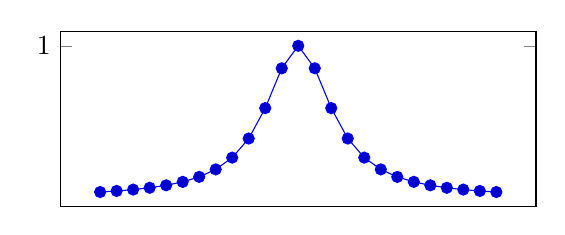
\begin{tikzpicture}
          \begin{axis}[width=3in, height=1.5in, ytick={1}, xtick=\empty]
            \addplot+[domain=-5:5] {1/(1 + x^2)};
          \end{axis}
        \end{tikzpicture}
      \end{center}
    \end{solution}

  \item Answer the following questions about 
  $\displaystyle A(x)=\int_0^x f(t)\,dt$; 
  Use Part
  1 of FTOC as appropriate.
  We know $\dfrac{d}{dx}A(x)=\fitb{1in}{f(x)}$.
  \begin{enumerate}
  \item
    \begin{problem}[\stretch{0.25}]
      For what value of $x$ is $A(x)=0$?
    \end{problem}

    \begin{solution}
      When $\boxed{x=0}$, definition, 
      $\displaystyle A(0) = \int_0^0 f(t)\,dt = 0$. 
    \end{solution}

  \item

    \note{They know from Math Ma that a function is increasing when its
      derivative is positive and decreasing when its derivative is
      negative; they may have trouble applying it in this case
      though.

      Some students may want to do this by visualizing $A(x)$ as
      $\displaystyle \int_0^x f(t)\,dt$; this usually leads to great
      confusion for negative $x$.}

    \begin{problem}[\stretch{0.5}]
      On what intervals is $A$ increasing?  Decreasing?  How do you
      know? 
    \end{problem}

    \begin{solution}
      $A$ is increasing when $A' > 0$ and decreasing when 
      $A' < 0$.  By FTOC 1, $A' = f$.  So, the previous sentence can
      be rewritten to say, ``$A$ is increasing when $f > 0$ and
      decreasing when $f < 0$.''  In this case, $f(x) = \frac{1}{1 + x^2}$
      is always positive, so $A$ is always increasing; that is,
      \fbox{$A$ is increasing on $(-\infty, \infty)$}.
    \end{solution}

  \item

    \note{They know from last semester that a function is concave up
      when its second derivative is positive and concave down when its
      second derivative is negative.}

    \begin{problem}[\stretch{0.5}]
      On what intervals is $A$ concave up?  Concave down?
    \end{problem}

    \begin{solution}
      $A$ is concave up when $A'' > 0$, and $A$ is concave
      down when $A'' < 0$.  By FTOC 1, $A'' = f'$.  So, the
      previous sentence can be rewritten to say ``$A$ is concave up
      when $f' > 0$ (in other words, when $f$ is increasing), and $A$
      is concave down when $f' < 0$ (in other words, when $f$ is
      decreasing).''  In this case, $f$ is increasing when $x < 0$ and
      decreasing when $x> 0$.  So, \fbox{$A$ is concave up on
        $(-\infty, 0)$ and concave down on $(0, \infty)$}.
    \end{solution}

  \item
    \begin{problem}[\stretch{2}]
      Sketch $A$.
    \end{problem}

    \begin{solution}
      We've seen that $A(0) = 0$; $A$ is always increasing; and
      $A$ is concave up on $(-\infty, 0)$ and concave down on $(0,
      \infty)$.  Therefore, its graph looks roughly like this:
      \begin{center}
        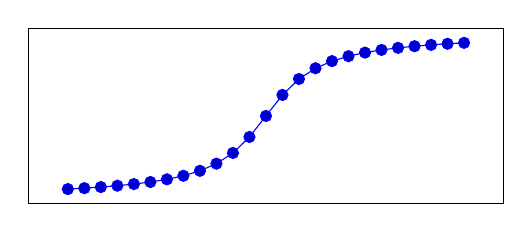
\begin{tikzpicture}
          \begin{axis}[xtick=\empty, ytick=\empty, width=3in, height=1.5in]
            \addplot+[domain=-5:5] {rad(atan(x))};
          \end{axis}
        \end{tikzpicture}
      \end{center}
    \end{solution}

  \item

    \note{This may be a good opportunity to bring up the idea that any two
    antiderivatives of $f$ must differ by a constant.  (If they believe
    this, then they can conclude that $A(x)$ really is $\arctan x$.)}

    \begin{problem}[\stretch{0.5}]
      Does your sketch remind you of a function you know?  Could 
      $A(x)$ actually be that function? Would that be consistent with
      what FTOC 1 tells you about $A(x)$?
    \end{problem}

    \begin{solution}
      The sketched graph looks like it could be $\arctan x$.  This would
      be consistent with FTOC 1, which tells us that $_0 A(x)$ is a
      function whose derivative is $\frac{1}{1 + x^2}$.  (After all,
      $\arctan x$ is a function whose derivative is $\frac{1}{1 + x^2}$.)

      In fact, since $_0 A(x)$ and $\arctan x$ have the same derivative,
      they must differ only by a constant; that is,
      \begin{equation}
        A(x) = \arctan x + C \text{ for some constant $C$}
      \end{equation}
      We can actually figure out what $C$ is by plugging in $x = 0$: $_0
      A(0) = \arctan 0 + C$.  Since we know that $A(0) = 0$ and
      $\arctan 0 = 0$, this tells us that $C = 0$.  Therefore,
      (1) says that $_0 A(x)$ really is $\arctan x$!  
    \end{solution}
    \end{enumerate}

  \item

    \note{Students should recognize that $B$ is a vertical shift of
      $A$, but they are often tempted to say that the vertical shift
      is 1.}

      Let $B(x)=\displaystyle\int_1^x f(t)\,dt$.
      
    \begin{enumerate}
    
    \item
    \begin{problem}[\stretch{0.1}]
        What is $\dfrac{d}{dx} B(x)$?
    \end{problem}

    \begin{solution}
        By FTOC 1, $\dfrac{d}{dx} B(x)
        =\dfrac{d}{dx} \displaystyle \int_1^x f(t)\,dt = f(x)$.
    \end{solution}

    \item
    \begin{problem}[\stretch{0.1}]
        For what value of $x$ is $B(x)=0$?
    \end{problem}

    \begin{solution}
        When $\boxed{x=1}$, by definition, 
        $B(1)=\displaystyle\int_1^1 f(t)\,dt=0$.
    \end{solution}

    \item 
    \begin{problem}[\newpage]
      Sketch $B$ on your graph in {{{{\#3}}(b)iv}}.  How does
      $B$ relate to $A$?
    \end{problem}

    \begin{solution}
      By {{{Problem Set 24}, {{\#6}}}}, $B(x)$ and $
      A(x)$ differ by a constant, so $B(x)$ is a 
      vertical shift of
      $A(x)$.  But how much do we need to shift $A(x)$ by?

      The key is that we know one $x$-intercept of $B(x)$, $x = 1$. So,
      to get the graph of $B(x)$, we shift the graph of $A(x)$
      up or down until it hits the $x$-axis at $x = 1$.  In this case, we
      must shift it down:
      \begin{center}
        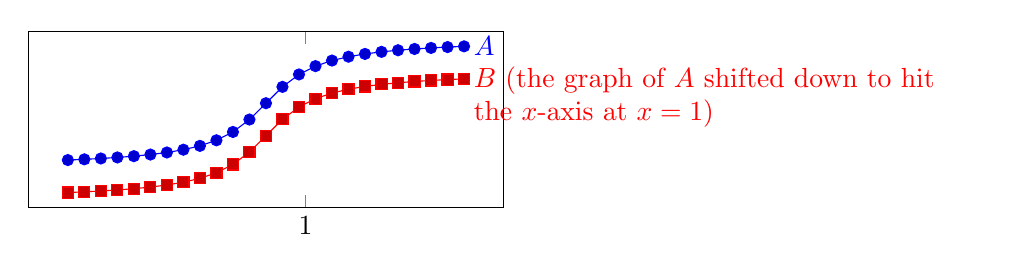
\begin{tikzpicture}
          \begin{axis}[xtick={1}, ytick=\empty, width=3in, height=1.5in,
            clip=false] 
            \addplot+[domain=-5:5] {rad(atan(x))} node[right] {$A$};
            \addplot+[domain=-5:5] {rad(atan(x)) - pi/4} node[anchor=north
            west, yshift=8pt, text
            width=2.5in] {$B$ 
            (the graph of $A$ shifted down to
              hit the $x$-axis at $x=1$)};
          \end{axis}
        \end{tikzpicture}
      \end{center}
      From the graphs, we can see that the amount we had to shift $A$
      down to get $B$ was exactly $A(1)$.  Since we found that
      $A(x) = \arctan x$, $A(1) = \arctan(1) = \frac{\pi}{4}$.
      So, we can conclude that $B(x) = A(x) - \frac{\pi}{4}$. 
    \end{solution}
    \end{enumerate}

  \end{enumerate}

\item 
  \note{This problem is mostly about notation.}

  \begin{enumerate}
  \item
    \begin{problem}[\stretch{0.5}]
      If $S(x) = \displaystyle \int_3^x \sin \left( \frac{\pi t^2}{2}
      \right)\,dt$, find $S'(x)$ and evaluate $S'(4)$.
    \end{problem}

    \begin{solution}
      If we write $\displaystyle f(t) = \sin \left( \frac{\pi
            t^2}{2} \right)$, then $S(x) = A(x)$, and FTOC 1 says
        that $A'(x) = f(x)$.  Therefore, $A'(4) = f(4) =
        \sin(8 \pi) = \boxed{0}$.
    \end{solution}

  \item
    \begin{problem}[\stretch{0.5}]
      Find $\displaystyle \frac{d}{dx} \left[ \int_3^x \sin \left(
          \frac{\pi t^2}{2} \right)\,dt \right]$. 
    \end{problem}

    \begin{solution}
      Using the same notation as in the previous part, this
        is asking for $\frac{d}{dx} \Big(A(x) \Big)$, which is
        simply $f(x) = \boxed{\sin \left( \frac{\pi x^2}{2} \right)}$ by
        FTOC 1.
    \end{solution}    

  \item

    \note{This is terrible notation, but it's important for students to
      realize that FTOC 1 only applies when they are integrating from a
      constant to $x$.}

    \begin{problem}[\stretch{0.5}]
      True or false: if $f$ is continuous on $[a, b]$, then $\displaystyle
      \frac{d}{dx} \left( \int_a^b f(x)\,dx \right) = f(x)$.
    \end{problem}

    \begin{solution}
      \fbox{False.}  $\displaystyle \int_a^b f(x)\,dx$ is a constant, so
      its derivative is $\boxed{0}$.  (Note that we generally consider
      $\displaystyle \frac{d}{dx} \left( \int_a^b f(x)\,dx \right)$ to be
      bad notation; it's not incorrect, but it's confusing: the
      $\frac{d}{dx}$ tells us we're thinking of $x$ as a variable, so it's
      better to use a different variable as the ``dummy variable'' in our
      integral.  So, it's better to write $\displaystyle \frac{d}{dx}
      \left( \int_a^b f(t)\,dt \right)$ or $\displaystyle \frac{d}{dx}
      \left( \int_a^b f(s)\,ds \right)$ to avoid confusion.)
    \end{solution}

  \end{enumerate}

\item  Let $f$ be the function whose graph is shown below.
       Let $A(x)=\displaystyle\int_8^x f(t)\,dt$. 

  \begin{tikzpicture}
    \begin{axis}[gridgraph, cycle list=black, ytick={-180, -120, ...,
        120}, width=2.6in, xlabel=$t$, minor xtick={1, 2, ..., 20}, minor
      ytick={-150, -90, ..., 90}, grid=both, tick style={black, thick}]
    \addplot+[sharp plot] coordinates { (0, 120) (5, 120) (15, -180) (20,
      -180) };
    \end{axis}
  \end{tikzpicture}

  \begin{enumerate}
  \item
    \begin{problem}[\vfill]
      For what values of $x$ in $(0, 20)$ is $A(x)$ increasing?
      Decreasing?
    \end{problem}

    \begin{solution}
      This depends on the sign of $A'(x)$, which is $f(x)$ by FTOC
      1.  In particular, $A(x)$ is increasing when $A'(x)
      = f(x)$ is positive and decreasing when $A'(x) = f(x)$ is
      negative.  Therefore, $A(x)$ is increasing on $(0, 9)$ and
      decreasing on $(9, 20)$.
    \end{solution}

  \item
    \begin{problem}[\vfill]
      For what values of $x$ is $A(x)$ concave up?  Concave down?
    \end{problem}

    \begin{solution}
      This depends on the sign of $A''(x)$, which is $f'(x)$ by
      FTOC 1.  In particular, $A(x)$ is concave up when $
      A''(x) = f'(x)$ is positive (which happens when $f$ is
      increasing), and $A(x)$ is concave down when $A''(x)
      = f'(x)$ is negative (which happens when $f$ is decreasing).  So,
      $A(x)$ is never concave up, and it's concave down on $(5,
      15)$.  (On $(0, 5)$ and $(15, 20)$, $f'(x) = 0$, so $A(x)$
      is linear.)
    \end{solution}

  \item
  \begin{problem}[\stretch{0.5}]
      Had our integral not been anchored at $8$ but instead at any
      number $a$ in the interval $(0,20)$, would that have changed
      the answers to parts (a) or (b)?
  \end{problem}

  \begin{solution}
      No, because $B(x)$ is simply a vertical shift of
      $A(x)$.
  \end{solution}

  \item
    \begin{problem}[\stretch{2.5}]
      Sketch the graph of $A(x)$. 
    \end{problem}

    \begin{solution}
      First, one $x$-intercept of $A(x)$ is $x = 8$ because
      $A(8) = 0$.  Based on the symmetry of the graph, we can also
      see that $A(10)=0$. Putting together what we've said already:
      \begin{itemize}
      \item On $(0, 5)$, $A(x)$ is increasing and linear (with
        slope $120$, since $A'(x) = f(x) = 120$).
      \item On $(5, 9)$, $A(x)$ is increasing and concave down.
      \item On $(9, 15)$, $A(x)$ is decreasing and concave down.
      \item On $(15, 20)$, $A(x)$ is decreasing and linear (with
        slope $-180$).  
      \end{itemize}
      That gives us the following graph:
      \begin{center}
        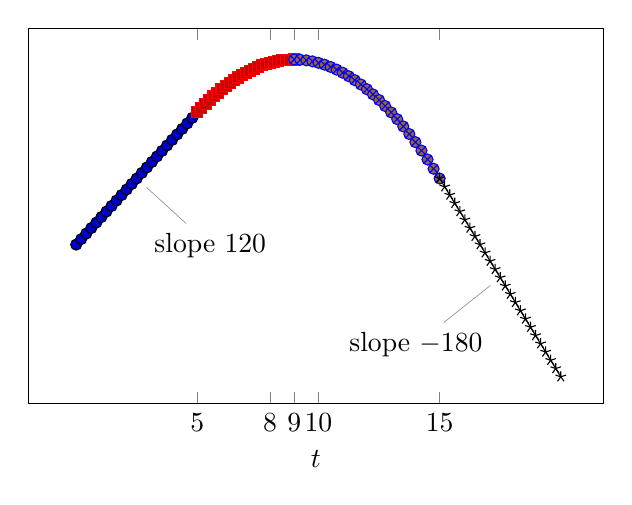
\begin{tikzpicture}
          \begin{axis}[enlargelimits=true, clip=false,
            width=3.5in, height=2.5in, xlabel=$t$, ymin=-1405, xtick={5,
              8, 9, 10, 15},
            ytick=\empty]
            \addplot+[black,domain=0:5] {120*x -825} node[pos=0.5,
            pin=-80:{slope 120}] {}; %
            \addplot+[red,domain=5:9] {-15 * (x^2 - 18*x + 25) - 825}; %
            \addplot+[blue,domain=9:15] {-15 * (x^2 - 18*x + 25) - 825};
            \addplot+[domain=15:20] {2175 - 180 * x} node[pos=0.5,
            pin=-100:{slope $-180$}] {}; %
          \end{axis}
        \end{tikzpicture}          
      \end{center}
      (Compare this with {{{{{{\#3}}(g)}} on {the worksheet ``The Definite Integral''}}}.)
    \end{solution}

  \end{enumerate}

\end{enumerate}
\end{document}